\subsection{Десятое БДЗ}

\setcounter{iii}{20}


\i\textbf{3.}\\
\pu
\begin{gather*}
   f_1(x) = x^2 + 6x - 9;\\
   f_2(x) = 2x - 4.\\
   \intertext{Сразу скажем, что точки пересечения этих кривых это $(-5; -14)$ и $(1; -2)$, поэтому нас будет интересовать только модуль разности интегралов этих функций на отрезке $[-5; 1]$.}
   \letus F_1 = \frac{x^3}{3} + 3x^2 - 9x,\ F_1 \in \int f_1(x) dx:\\
   \int_{-5}^1 f_1(x)dx = F_1(1) - F_1(-5) = -84;\\
   \letus F_2 = x^2 - 4x,\ F_2 \in \int f_2(x) dx:\\
   \int_{-5}^1 f_2(x)dx = F_2(1) - F_2(-5) = -48;\\
   S = \abs{\int_{-5}^1 f_1(x)dx - \int_{-5}^1 f_2(x)dx} = 36.
\end{gather*}
\pu
\begin{gather*}
    r = 2\sin(4\phi).
    \intertext{В силу того, что нас инетересует только одна петля кривой, мы будем рассматривать только начения $\phi$ на отрезке $[0, \frac{\pi}{4}]$, тогда искомую площадь мы сможем найти как}
    \frac{1}{2}\int_0^{\pi/4} r^2(\phi) d\phi = 
    2\int_0^{\pi/4} \sin^2(4\phi) d\phi;\\
    \letus \psi = 4\phi, d\psi = 4d\phi:\\
    \frac{1}{2}\int_0^\pi \sin^2(\psi)d\psi = 
    \frac{1}{2}\int_0^\pi \brackets{\frac{1}{2} - \frac{1}{2}\cos(2\psi)}dx = \frac{\pi}{4} + 0.\\
    S = \frac{\pi}{4}.
\end{gather*}


\i\textbf{8.}
\begin{gather*}
    f(x) = \frac{\sqrt{x^3}}{\sqrt[4]{1-x^2}};\ x \in [1; \frac{1}{2}].
    \intertext{Мы знаем, что объём тела врещинея можно вычислить по формуле}
    V = \pi\int_0^{1/2}f(x)^2dx = \pi\int_0^{1/2} \frac{x^3}{\sqrt{1-x^2}};\\
    \letus t = x^2,\ dt = 2xdx:\\
    V = \frac{\pi}{2}\int_0^{1/4} \frac{t}{\sqrt{1-t}}dt;\\
    \letus s = 1-t,\ ds = -dt:\\
    V = -\frac{\pi}{2}\int_1^{3/4} \frac{1-s}{\sqrt{s}}ds = 
    -\frac{\pi}{2}\int_1^{3/4} \brackets{\frac{1}{\sqrt{s}} - \sqrt{s}}ds = 
    -\frac{\pi}{2}\int_{3/4}^1 \brackets{\frac{1}{\sqrt{s}} - \sqrt{s}}ds = \\ = 
    -\frac{\pi}{2}\int_{3/4}^1 \sqrt{s}ds + \frac{\pi}{2}\int_{3/4}^1 \frac{ds}{\sqrt{s}} = 
    \brackets{\frac{\pi s^{3/2}}{3}}\bigg|_{3/4}^1 + \brackets{\pi \sqrt{s}}\bigg|_{3/4}^1.\\
    V = \brackets{\frac{2}{3} - \frac{3\sqrt{3}}{8}}\pi.
\end{gather*}


\i\textbf{6.}

\begin{wrapfigure}[]{r}{0pt}
    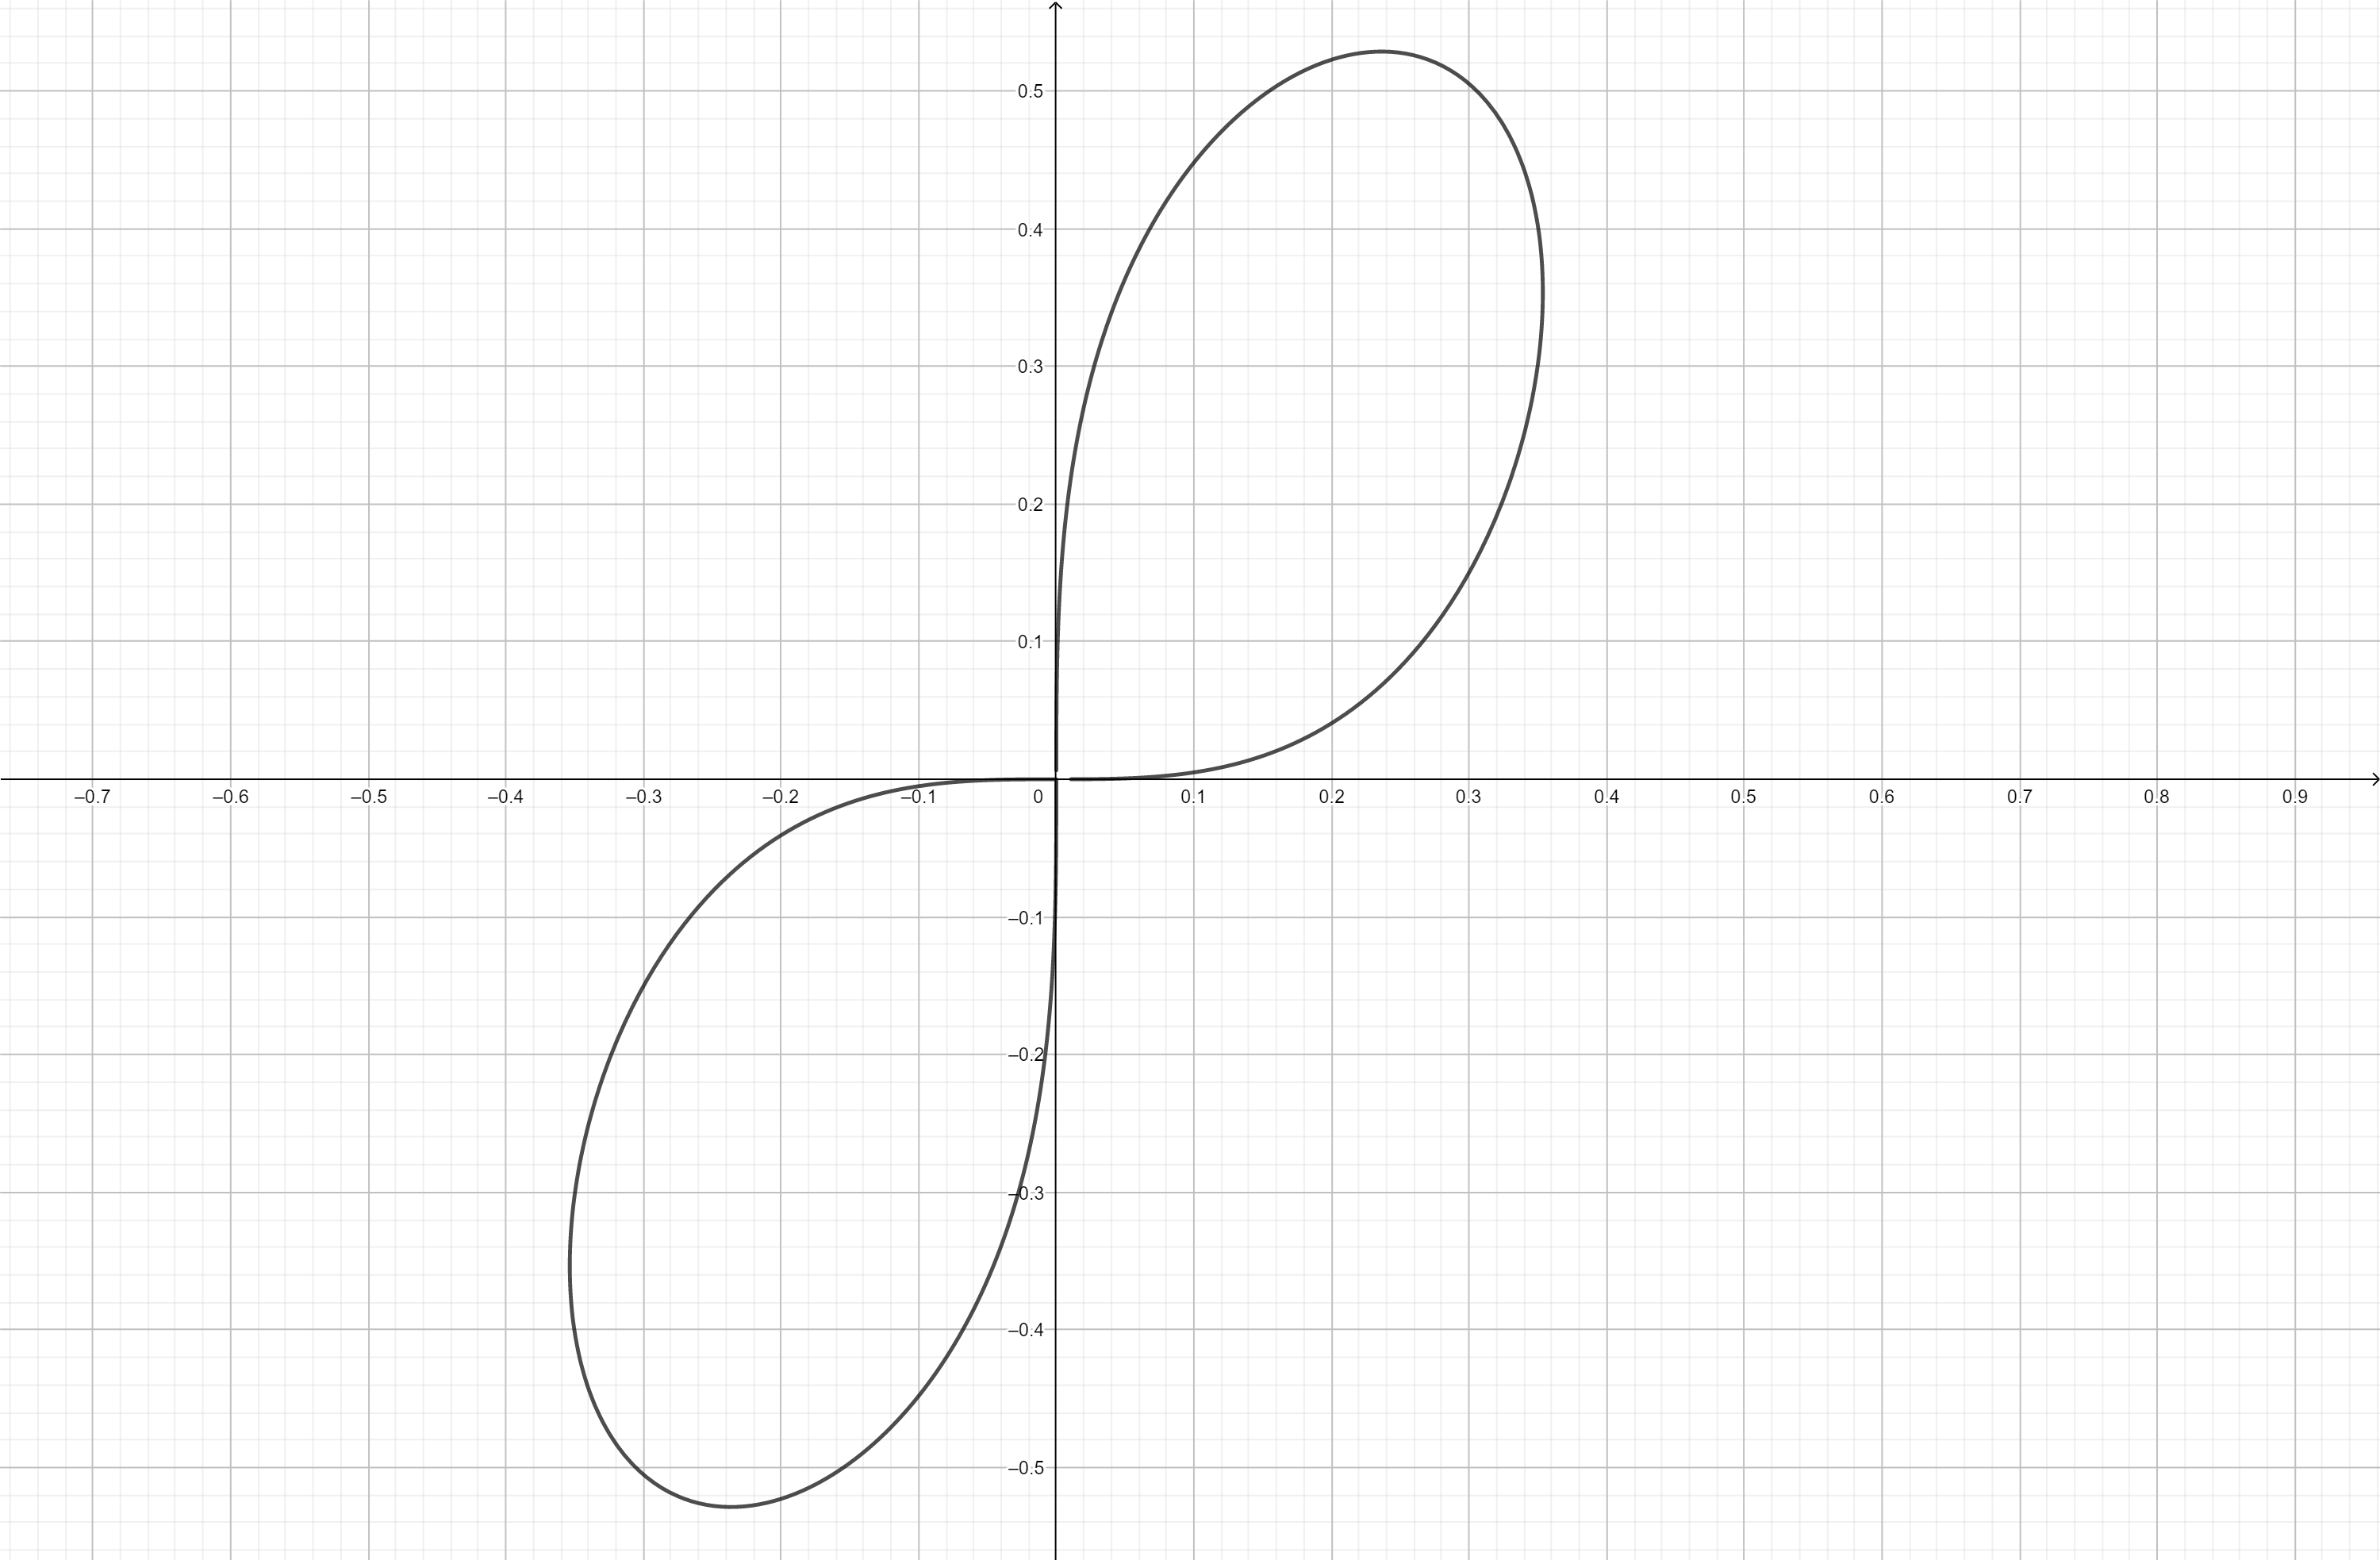
\includegraphics[scale=6]{course1/calculus/homeworks/some data/05.23.png}
\end{wrapfigure}
Как мы видим, наша кривая делает 2 петли, посчитаем площадь той из них, которая получается при $x \geq 0$. Зададим нашу кривую в полярных координатах, в этом случае она должна удовлетворять уравнению (\textcolor{red}{\ref{param}}). При этом нас будет интересовать только та часть этой кривой, которая получается при $\phi \in [0; \frac{\pi}{2}]$ и $r > 0$. Тогда мы с вами получим, что нам нужно найти площадь сектора, который задаётся уравнением $r = \sqrt{\frac{\sin(\phi)\cos(\phi)}{4\cos^3(\phi) + 1}}$ на отрезке $[0, \frac{\pi}{2}]$.
\begin{gather*}
    4r^4\cos^4(\phi) + r^4(\cos^2(\phi) + \sin^2(\phi))^2 = r^2\sin(\phi)\cos(\phi);\\
    4r^4\cos^4(\phi) + r^4 = r^2\sin(\phi)\cos(\phi);\\
    r^2 = \frac{\sin(\phi)\cos(\phi)}{4\cos^4(\phi) + 1}. \tag{\textcolor{red}{1}} \label{param}
\end{gather*}
Теперь займёмся подсчётом нужно интеграла.
\begin{gather*}
    S = \frac{1}{2}\int_0^{\pi/2} r^2(\phi)d\phi = \frac{1}{2}\int_0^{\pi/2} \frac{\sin(\phi)\cos(\phi)}{4\cos^4(\phi) + 1}d\phi;
    \letus t = \cos(\phi),\ dt = -\sin(\phi):\\
    S = \frac{1}{2}\int_0^1 \frac{t}{4t^4 + 1}dt;\\
    \letus s = (2t)^2,\ ds = 4tdt:\\
    S = \frac{1}{8}\int_0^2 \frac{1}{s^2+1}ds = \frac{1}{8}\arctan(s)\bigg|_0^2 = \frac{1}{8}\arctan(2).
\end{gather*}


\i\textbf{2.}
\begin{gather*}
    \begin{cases}
        x = t - \sin(t),\\
        y = 1 - \cos(t),\ t \in [0, 2\pi];
    \end{cases}
    \intertext{как известно, длину кривой можно посчитать по формуле}
    L = \int_0^{2\pi} \sqrt{x\hatch^2 + y\hatch^2}dt = \int_0^{2\pi} \sqrt{(1-\cos(t))^2 + \sin^2(t)}dt = \int_0^{2\pi} \sqrt{2 - 2\cos(t)}dt = \\ = 
    2\int_0^{2\pi} \sqrt{\sin^2\brackets{\frac{t}{2}}}dt = 2\int_0^{2\pi} \abs{\sin\brackets{\frac{t}{2}}};\\
    \letus s = \frac{t}{2},\ ds = \frac{1}{2}dt:\\
    L = 4\int_0^\pi \abs{\sin(s)}ds = 4\int_0^\pi \sin(s)ds = (-4\cos(s))\bigg|_0^\pi = 8.
\end{gather*}


\i\textbf{5.}\\
\pu Если интеграл сходится, то его можно посчитать по формуле
\begin{gather*}
    \int_0^\infty \frac{dx}{x\ln(x)} = \limit{m}{\infty}\int_0^m \frac{dx}{x\ln(x)}.
\end{gather*}
Однако, при $m \geq 1$ отрезок $[0, m]$ содержит точку разрыва второго рода с пределами $\pm \infty$, так что интеграл не считается, а значит, нельзя определить предел, поэтому данный интеграл расходится.

\pu Если интеграл сходится, то его можно посчитать по формуле
\begin{gather*}
    \int_0^{\sqrt{3/\pi}} \frac{1}{x^2}\sin\brackets{\frac{1}{x}}dx = \limit{\epsilon}{0+}\int_\epsilon^{\sqrt{{3/\pi}}} \frac{1}{x^2}\sin\brackets{\frac{1}{x}}dx.
    \intertext{Посчитаем неопределённый интеграл для подстановки в формулу Ньютона Лейбница:}
    \int \frac{\sin\brackets{\frac{1}{x}}}{x^2}dx;\\
    \letus t = \frac{1}{x},\ dt = -\frac{1}{x^2}dx:\\
    -\int \sin(t)dt = \cos(t) + C = \cos\brackets{\frac{1}{x}} + C.\\
    \intertext{Положим $F = \cos\brackets{\frac{1}{x}} \in \int \frac{\sin\brackets{\frac{1}{x}}}{x^2}dx$, тогда желаемый интеграл можно посчитать по формуле}
    \int_0^{\sqrt{3/\pi}} \frac{1}{x^2}\sin\brackets{\frac{1}{x}}dx = \limit{\epsilon}{0+} \cos\brackets{\frac{1}{x}}\bigg|_\epsilon^{\sqrt{3/\pi}} = \cos\brackets{\frac{1}{\sqrt{3/\pi}}} - \limit{0+}{\epsilon} \cos\brackets{\frac{1}{\epsilon}}.
    \intertext{Легко заметить, что предел в последнем выражении не считается, а значит, данный интеграл расходится.}
\end{gather*}